\documentclass[10pt,a4paper]{article}
\usepackage[utf8]{inputenc}
\usepackage[english]{babel}
%\usepackage{minted}
\usepackage{listings}
\usepackage{xcolor}
\usepackage{graphicx}

%For syntax highlighting
\definecolor{codegreen}{rgb}{0,0.6,0}
\definecolor{codegray}{rgb}{0.5,0.5,0.5}
\definecolor{codepurple}{rgb}{0.58,0,0.82}
\definecolor{backcolour}{rgb}{1,1,1}

%%Sets different parameters
\lstdefinestyle{mystyle}{
	backgroundcolor=\color{backcolour},   
    commentstyle=\color{codegreen},
    keywordstyle=\color{magenta},
    numberstyle=\tiny\color{codegray},
    stringstyle=\color{codepurple},
    basicstyle=\ttfamily\footnotesize,
    breakatwhitespace=false,         
    breaklines=true,                 
    captionpos=b,                    
    keepspaces=true,                 
    numbers=left,                    
    numbersep=5pt,                  
    showspaces=false,                
    showstringspaces=false,
    showtabs=false,                  
    tabsize=4
}
\lstset{style=mystyle}

\title{\bf Sorting}
\author{\vspace{-10ex}}
\date{\vspace{-10ex}}
\begin{document}
\maketitle

\begin{minipage}{0.45\textwidth}
        \begin{tabular}{l l}
            \textbf{Expt No:}&6\\
            \textbf{Date :}&09/10/2020
        \end{tabular}
\end{minipage}%
\begin{minipage}{0.45\textwidth}
        \begin{tabular}{l l}
             \textbf{Name:}& Shivanirudh S G  \\
             \textbf{Reg No:} & 185001146 
        \end{tabular}
\end{minipage}
\vspace{1cm}
\hrule

\begin{flushleft}
\subsection*{\textbf{Aim:}} 
To perform sorting operations in 8086.

\vspace{1cm}
\hrule
\subsection*{\textbf{\underline{Ascending Order}}}

\subsubsection*{\textbf{Algorithm:}}
\begin{itemize}
    \item Move the data segment to the AX register and then move it to the DS register.
    \item Move value of count to CL register.
    \item Move offset of arr into SI register under label OUTER.
    \item Move value of count to CH register.
    \item Move value at [SI] to AL register, [SI+1] to AH register, under label INNER.
    \item Compare AH, AL with CMP AH, AL.
    \item If CF = 0, jump to label NOSWAP. 
    \item Swap values of AH, AL with XCHG AH, AL
    \item Move value in AL to [SI] register, AH to [SI+1].
    \item Increment SI, decrement CH under label NOSWAP.
    \item Jump to INNER if ZF = 0.
    \item Decrement CL and jump to OUTER if ZF = 0.
\end{itemize}

\newpage
\subsubsection*{\textbf{Program:}}

\begin{table}[htb]
\centering
\resizebox{\columnwidth}{!}{
\begin{tabular}{|l|l|} 
\hline
\textbf{Program}                                                 & \textbf{Comments}                             \\ 
\hline
\hline
assume cs:code, ds:data                                          & Declare code and data segments                \\
\hline
data segment                                                     & Start of data segment                         \\
\hline
arr db 05H, 04H, 03H, 02H, 01H                                   & Define array of values arr                    \\
\hline
count db 04H                                                     & Define byte count with hex value 04           \\
\hline
data ends                                                        & End of data segment                           \\
\hline
code segment                                                     & Start of code segment                         \\
\hline
start:~mov ax, data                                              & Move data to AX register                      \\
\hline
mov ds, ax                                                       & Move contents of AX register to DS register   \\
\hline
mov cl, count                                                    & Move value of count to CL register            \\
\hline
outer:~mov si, offset arr                                        & Move offset of arr to SI register             \\
\hline
mov ch, count                                                    & Move value of count to CH register            \\
\hline
inner:~mov al, [si]                                              & Move value at offset in SI to AL register     \\
\hline
mov ah, [si+1]                                                   & Move value at offset in SI register +1 to AH  \\
\hline 
cmp ah, al                                                       & Compare values in AH, AL registers            \\
\hline
jnc noswap                                                       & Jump to NOSWAP if CF = 0                      \\
\hline
xchg al, ah                                                      & Swap values in AL, AH registers               \\
\hline
mov [si], al                                                     & Move value in AL register to offset at [SI]   \\
\hline
mov [si+1], ah                                                   & Move value in AH register to offset at [SI]+1 \\
\hline
noswap:~inc si                                                   & Increment value of SI                         \\
\hline
dec ch                                                           & Decrement value of CH                         \\
\hline
jnz inner                                                        & Jump to INNER if ZF = 0                       \\
\hline
dec cl                                                           & Decrement value of CL                         \\
\hline
jnz outer                                                        & Jump to OUTER if ZF = 0                       \\
\hline
mov ah, 4ch                                                & To request interrupt                          \\
\hline
int 21h                                                          & Request interrupt routine                     \\ 
\hline
code ends                                                        & End of code segment                           \\
\hline
end start                                                        &                                               \\
\hline
\end{tabular}
}
\end{table}

\newpage
\subsection*{\textbf{Unassembled code:}}
\begin{figure}[h]
    \centering
    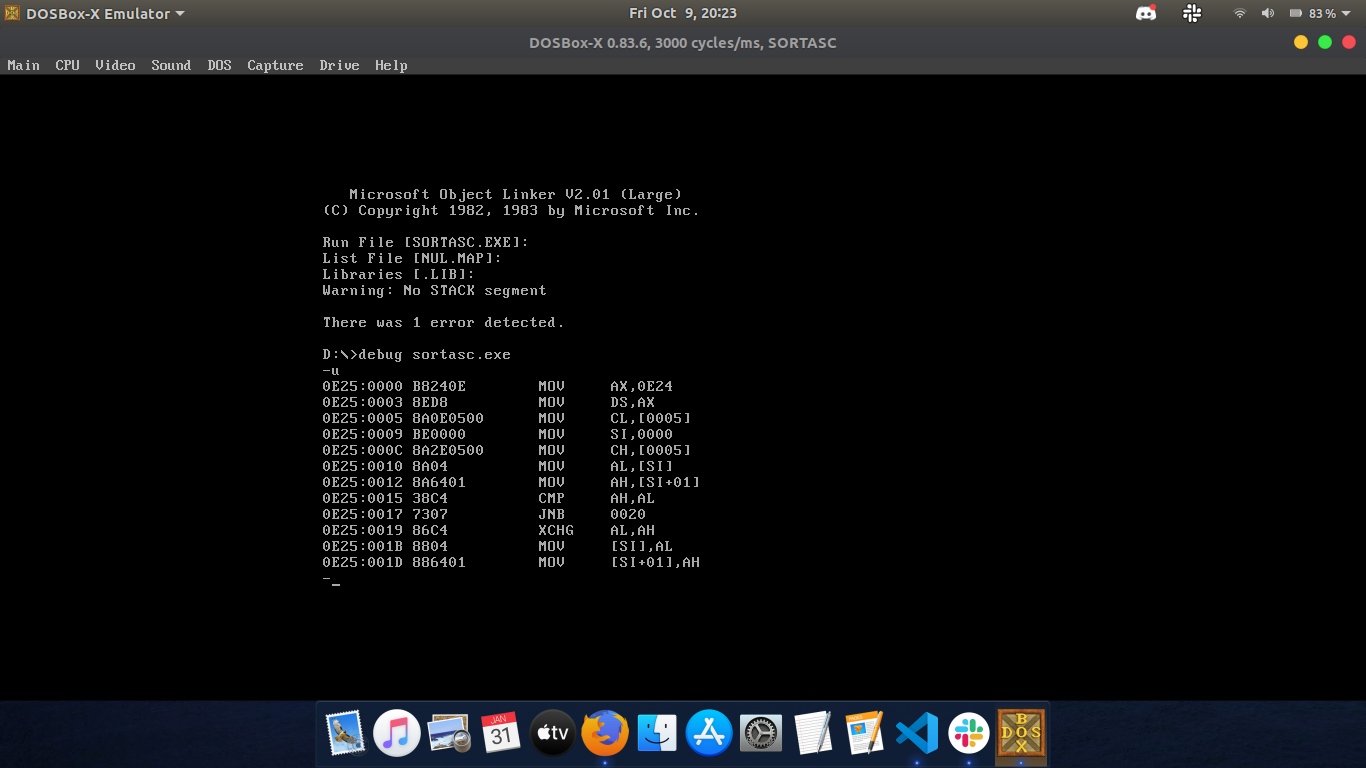
\includegraphics[trim = 100mm 60mm 200mm 120mm, clip, width = \textwidth]{Pics/SAUS.png}
\end{figure}
\subsubsection*{\textbf{Input and Output:}}
\begin{figure}[h]
    \centering
    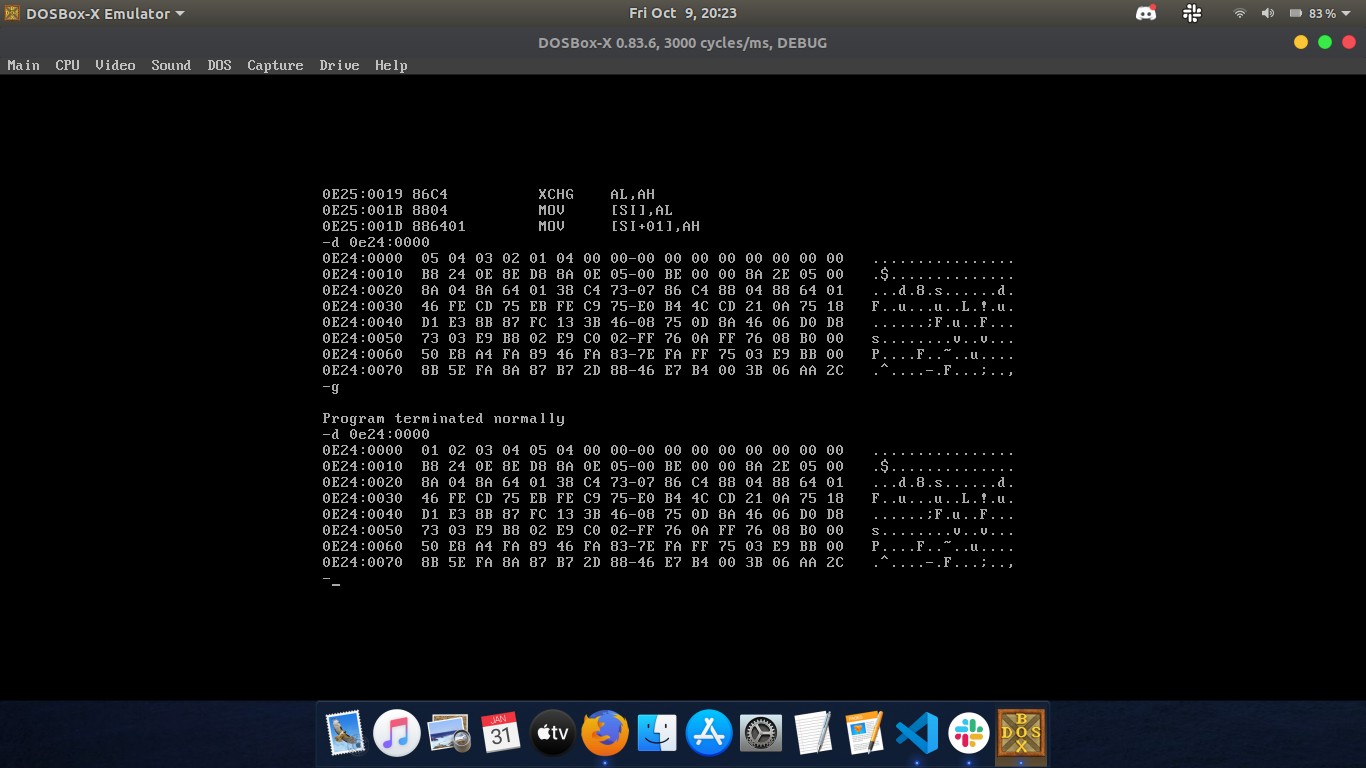
\includegraphics[trim = 100mm 60mm 100mm 80mm, clip, width = \textwidth]{Pics/SAIO.png}
    \caption{ \textbf{Input:} 05H, 04H, 03H, 02H, 01H; \newline \hspace{1cm}
              \textbf{Output:} 01H, 02H, 03H, 04H, 05H}
\end{figure}
%-------------------------------------------------------------------------------------------------------------------------------------------
\hrule
\newpage
\subsection*{\textbf{\underline{Descending Order}}}

\subsubsection*{\textbf{Algorithm:}}
\begin{itemize}
    \item Move the data segment to the AX register and then move it to the DS register.
    \item Move value of count to CL register.
    \item Move offset of arr into SI register under label OUTER.
    \item Move value of count to CH register.
    \item Move value at [SI] to AL register, [SI+1] to AH register, under label INNER.
    \item Compare AH, AL with CMP AH, AL.
    \item If CF = 1, jump to label NOSWAP. 
    \item Swap values of AH, AL with XCHG AH, AL
    \item Move value in AL to [SI] register, AH to [SI+1].
    \item Increment SI, decrement CH under label NOSWAP.
    \item Jump to INNER if ZF = 0.
    \item Decrement CL and jump to OUTER if ZF = 0.
\end{itemize}

\newpage
\subsubsection*{\textbf{Program:}}

\begin{table}[htb]
\centering
\resizebox{\columnwidth}{!}{
\begin{tabular}{|l|l|} 
\hline
\textbf{Program}                                                 & \textbf{Comments}                             \\ 
\hline
\hline
assume cs:code, ds:data                                          & Declare code and data segments                \\
\hline
data segment                                                     & Start of data segment                         \\
\hline
arr db 05H, 04H, 03H, 02H, 01H                                   & Define array of values arr                    \\
\hline
count db 04H                                                     & Define byte count with hex value 04           \\
\hline
data ends                                                        & End of data segment                           \\
\hline
code segment                                                     & Start of code segment                         \\
\hline
start:~mov ax, data                                              & Move data to AX register                      \\
\hline
mov ds, ax                                                       & Move contents of AX register to DS register   \\
\hline
mov cl, count                                                    & Move value of count to CL register            \\
\hline
outer:~mov si, offset arr                                        & Move offset of arr to SI register             \\
\hline
mov ch, count                                                    & Move value of count to CH register            \\
\hline
inner:~mov al, [si]                                              & Move value at offset in SI to AL register     \\
\hline
mov ah, [si+1]                                                   & Move value at offset in SI register +1 to AH  \\
\hline 
cmp ah, al                                                       & Compare values in AH, AL registers            \\
\hline
jc noswap                                                        & Jump to NOSWAP if CF = 1                      \\
\hline
xchg al, ah                                                      & Swap values in AL, AH registers               \\
\hline
mov [si], al                                                     & Move value in AL register to offset at [SI]   \\
\hline
mov [si+1], ah                                                   & Move value in AH register to offset at [SI]+1 \\
\hline
noswap:~inc si                                                   & Increment value of SI                         \\
\hline
dec ch                                                           & Decrement value of CH                         \\
\hline
jnz inner                                                        & Jump to INNER if ZF = 0                       \\
\hline
dec cl                                                           & Decrement value of CL                         \\
\hline
jnz outer                                                        & Jump to OUTER if ZF = 0                       \\
\hline
mov ah, 4ch                                                & To request interrupt                          \\
\hline
int 21h                                                          & Request interrupt routine                     \\ 
\hline
code ends                                                        & End of code segment                           \\
\hline
end start                                                        &                                               \\
\hline
\end{tabular}
}
\end{table}

\newpage
\subsection*{\textbf{Unassembled code:}}
\begin{figure}[h]
    \centering
    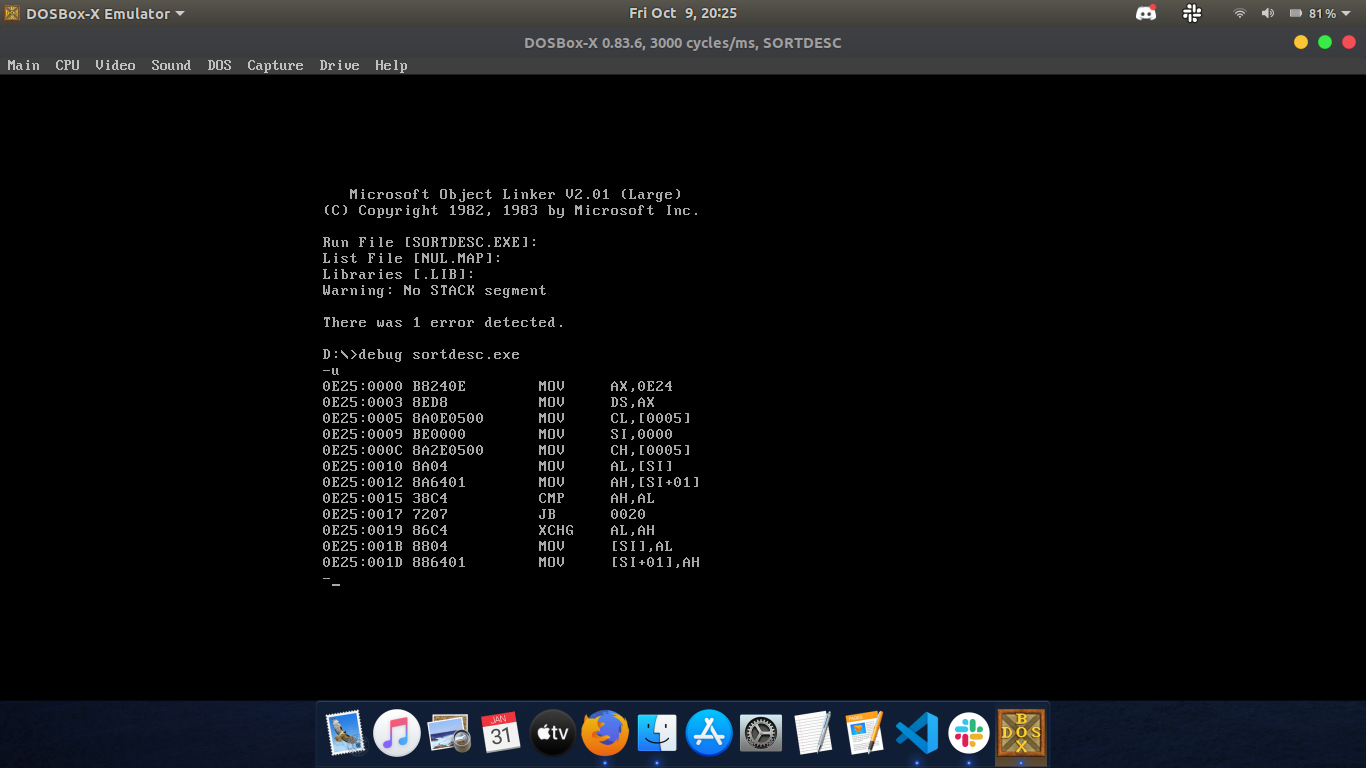
\includegraphics[trim = 100mm 60mm 200mm 120mm, clip, width = \textwidth]{Pics/SDUS.png}
\end{figure}
\subsubsection*{\textbf{Input and Output:}}
\begin{figure}[h]
    \centering
    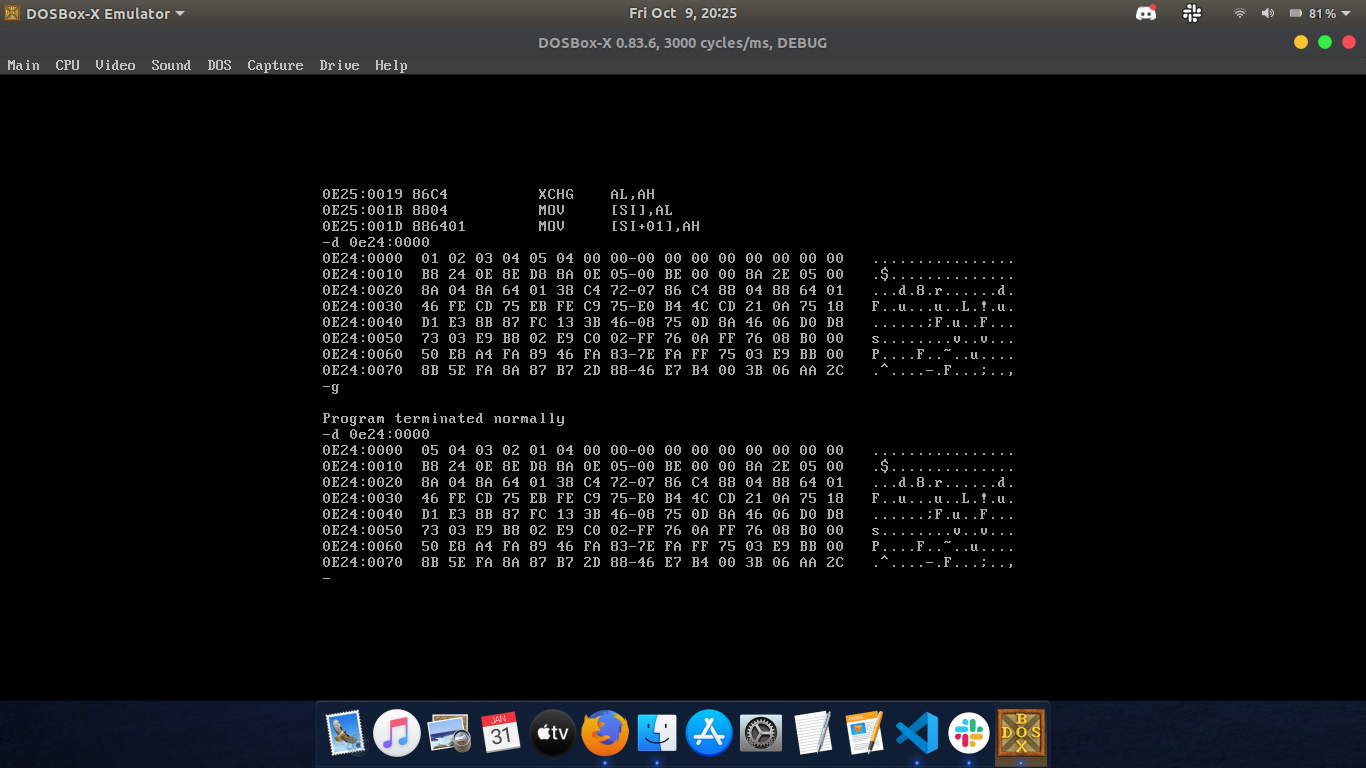
\includegraphics[trim = 100mm 60mm 100mm 80mm, clip, width = \textwidth]{Pics/SDIO.png}
    \caption{ \textbf{Input:} 01H, 02H, 03H, 04H, 05H; \newline \hspace{1cm}
              \textbf{Output:} 05H, 04H, 03H, 02H, 01H}
\end{figure}
\hrule
\subsection*{\textbf{Result:}}
The 8086 programs were written to perform matrix operations, and the results observed.
\end{flushleft}
\end{document}